\documentclass[a4paper,10pt]{article}

%\usepackage{subfig}
\usepackage{caption}
\usepackage{subcaption}
\usepackage{float}
\usepackage{graphicx}
\usepackage{verbatim}
\usepackage{amsthm}
\usepackage{amsmath}
\usepackage{amssymb}
\usepackage{geometry}


\newtheorem{defn}{Definition}
\newtheorem{prop}{Proposition}
\newtheorem{theorem}{Theorem}
\newtheorem{cor}{Corollary}

%opening
\title{Opinion-dependent Rewiring Model}
\author{Sam Magura, Vitchyr Pong}

\begin{document}

\maketitle
\section{Model Definition}
The process operates on a graph $G = (V, E)$. Each vertex $v = \langle v_1, v_2, \ldots, v_D \rangle$ where $v_1$, $v_2$, and so on represent the opinions of $v$. Initially, each vertex is placed randomly in the \emph{opinion space} $\Omega = [0, 1]^D$. The distance function $d(x, y)$ gives the \emph{opinion distance} between two vertices $x$ and $y$. We use
\begin{equation}
 d(x, y) = |x_1 - y_1| + |x_2 - y_2| + \ldots.
\end{equation}
Let the constant $p = 1 / D$ so that $p \; d(x, y) \leq 1$ for any possible $\{x, y\}$.  
\\\\Each iteration, do the following.
\begin{enumerate}
 \item Randomly choose an edge from the graph.
 \item Apply a random orientation $(x, y)$ to the edge.
 \item Let $k(x)$ give the degree of $x$. If $k(x) = n - 1$, do nothing this iteration.
 \item \label{item:z} Randomly choose a vertex $z$ from the set of all vertices that are neither $x$ nor adjacent to $x$.
 \item With probability
 \begin{equation}
 \label{exp:pr}
  p \; d(x, y) \; \min\left(1, \frac{d(x, y)}{d(x, z)}\right), 
 \end{equation}
remove the edge $\{x, y\}$ and add the edge $\{x, z\}$. 
\end{enumerate}
In Expression \ref{exp:pr}, $p \; d(x, y)$ represents the chance that $\{x, y\}$ is marked for removal and $\min(1, \frac{d(x, y)}{d(x, z)})$ represents the chance that the addition of $\{x, z\}$ is accepted. We say ``$\{x, y\}$ is marked for removal'' since the edge is only removed if the addition of $\{x, z\}$ is also accepted. Thus, the greater the opinion distance of the original edge $\{x, y\}$, the greater the chance that that edge is marked for removal. The addition of the new edge $\{x, z\}$ is always accepted if the new distance is less than the original distance. However, if the new distance is greater, the addition is accepted with probability $d(x, y) / d(x, z).$

In many network models, multiple edges are allowed because they are relatively unlikely in large networks. However, if multiedges are allowed in this model, many edges will accumulate between pairs of vertices that have especially low opinion distances. Because of this, we prevent the creation of multiedges by refusing to select a $z$ that is already to adjacent to $x$ in Step \ref{item:z}.

\section{Stationary Distribution}
The model is a Markov Chain because the probability of transitioning from a state $G$ to a state $H$ is dependent only $G$ and $H$. 

\begin{defn}
 Graphs $G = (V, E_G)$ and $H = (V, E_H)$ are the same state in the Markov Chain if and only if $E_G = E_H$.
\end{defn}


\paragraph{Transition probability} Consider states $G$ and $H$ such that $\{x, y\}$ is in $G$ but not $H$, and $\{x, z\}$ is in $H$ but not $G$. For a transition from $G$ to $H$, the following must occur.
\begin{enumerate}
 \item The edge $\{x, y\}$ is selected. This occurs with probability $\frac{1}{m}$.
 \item The orientation $(x, y)$ is chosen. This occurs with probability $\frac{1}{2}$.
 \item Vertex $z$ is selected in Step \ref{item:z} of the model definition. This occurs with probability $\frac{1}{m - k(x) - 1}$ where $k(x)$ gives the degree of $x$, since $z$ is selected randomly from the set of all vertices that are neither $x$ nor adjacent to $x$.
 \item The rewiring is accepted. This occurs with probability $ p \; d(x, y) \; \min(1, \frac{d(x, y)}{d(x, z)}).$
\end{enumerate}
Therefore the transition probability is 

\begin{equation}
\label{eqn:pgh}
 P(G, H) = \frac{ p \; d(x, y) \; \min\left(1, \frac{d(x, y)}{d(x, z)}\right)}{2m \left(m - k(x) - 1\right)}.
\end{equation}

\begin{theorem}
  The detailed balance condition is satisfied by the stationary distribution
\begin{equation}
 \pi(G) = b \prod_{e} \frac{1}{d(e)^2}
\end{equation}
where $b$ is some normalization coefficient, $e$ is any edge in graph $G$, and $d(e)$ gives the distance between the endpoints of edge $e$.
\end{theorem}
\begin{proof}
 The detailed balance condition is
 \begin{equation}
 \pi(G) \: P(G, H) = \pi(H) \: P(H, G).
\end{equation}
Without loss of generality, suppose $d(x, y)$ is greater than $d(x, z)$. Substituting in the transition probabilities from Equation \ref{eqn:pgh} and the proposed stationary distribution $\pi$, we have

\begin{equation}
\frac{ p \; d(x, y)}{2m \left(m - k(x) - 1\right)}
\left(b\prod_{e \in E_G} \frac{1}{d(e)^2}\right) =
\frac{ p \; d(x, z)^2}{2m \; d(x, y) \left(m - k(x) - 1\right)}\:
\left(b\prod_{e \in E_H} \frac{1}{d(e)^2}\right).
\end{equation}
This simplifies to
\begin{equation}
d(x, y)^2 \prod_{e \in E_G} \frac{1}{d(e)^2} =
d(x, z)^2 \prod_{e \in E_H} \frac{1}{d(e)^2}
\end{equation}
since the degree of $x$ does not change. Because the only difference between $G$ and $H$ is that $G$ has an edge $\{x, y\}$ that $H$ does not and $H$ has an edge $\{x, z\}$ that $G$ does not, the detailed balance condition holds for the proposed stationary distribution $\pi$.
\end{proof}

\section{Constructive Model}
\begin{theorem}
\label{thm:perc}
When the rewiring model has reached the steady state, the probability that an edge $e^*$ is present is approximately
\begin{equation*}
 \frac{c}{d(e^*)^2 + c}
\end{equation*}
where $c$ is the constant that satisfies
\begin{equation}
\label{eqn:c}
 \sum_{e \in K_n} \frac{c}{d(e)^2 + c} = m.
\end{equation}
$K_n$ is the complete graph on $n$ vertices, $n = |V|$, and $m = |E|$.
\end{theorem}
\begin{proof}
For a constructive model in which each edge $e$ is independently present with probability $P(e)$, the probability that a particular graph $G$ is produced is
\begin{equation}
 \mu(G) = \prod\limits_{e \in G} \frac{P(e)}{1 - P(e)} \prod\limits_{e \in K_n} (1 - P(e)).
\end{equation}
We want to find the function $P(e)$ such that $\mu(G)$ is approximately equal to $\pi(G)$. Because the expressions for $\mu(G)$ and $\pi(G)$ both contain a product over all edges $e \in G$ multiplied by some factor which is independent of $G$, we can write
\begin{equation}
\label{eqn:proportional}
 \frac{P(e)}{1-P(e)} \propto \frac{1}{d(e)^2} \;\;\;\;\longrightarrow\;\;\;\; P(e) = \frac{c}{d(e)^2 + c}.
\end{equation}
Since each state in the rewiring model contains exactly $m$ edges, the expected the number of edges of a graph produced by the constructive model should be $m$:
\begin{equation}
\label{eqn:sum-to-m}
 \sum_{e \in K_n} P(e) = m.
\end{equation}
We reach our criterion for $c$ by substituting Equation \ref{eqn:proportional} into Equation \ref{eqn:sum-to-m}.
\end{proof}

\begin{figure}
 \centering
 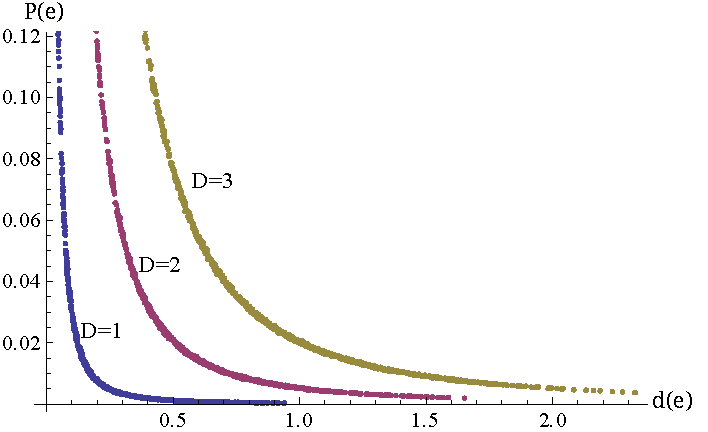
\includegraphics{images/edge_existence2.pdf}
 \caption{Experimental verification of Theorem \ref{thm:perc} using data from our implementation of the rewiring model. Each datapoint is for a different edge in the complete graph $K_{50}$. The datapoints do in fact lie on curves of the form $\frac{c}{d(e)^2 + c}$.}
\end{figure}

\begin{prop}
\label{prop:c}
For large $n$, $c$ satisfies
 \begin{equation*}
  \int\limits_\Omega \int\limits_\Omega \frac{du \, dv}{d(u, v)^2 + c} = \frac{2m}{c\,n^2}.
 \end{equation*}
where $\Omega$ is the opinion space $[0, 1]^D$.
\end{prop}
\begin{proof}
 Equation \ref{eqn:c} can be rewritten as
 \begin{equation}
 \label{eqn:double-sum}
  \frac{1}{2} \sum\limits_{u}\sum\limits_{v \neq u} \frac{c}{d(u, v)^2 + c} = m
 \end{equation}
 where $u$ and $v$ are any vertices in the graph. For large $n$, vertices are evenly distrbuted within the opinion space since they are placed randomly. Therefore, there are $n \,du$ vertices in an interval $du$ with dimensions $du_1, du_2, \ldots, du_D$, and $\frac{1}{2}(n\, du)(n\, dv)$ edges between vertices in $du$ and vertices in $dv$. Because the sums in Expression \ref{eqn:double-sum} are computed over $n$ and $n - 1$ vertices respectively, and $n$ is large, we can express the two sums as a double integral:
 \begin{equation}
  \frac{c\,n^2}{2} \int\limits_\Omega \int\limits_\Omega \frac{du \, dv}{d(u, v)^2 + c} = m.
 \end{equation}
\end{proof}
\begin{prop}
\label{prop:c1D}
 For $D=1$ and large $n$,
 \begin{equation*}
  \frac{2}{\sqrt{c}}\,\tan^{-1} \frac{1}{\sqrt{c}} + \ln\frac{c}{c+1} = \frac{2m}{c\,n^2}.
 \end{equation*}
\end{prop}
\begin{proof}
For $D=1$, the double integral in Theorem \ref{prop:c} reduces to
 \begin{equation}
  \frac{c\,n^2}{2} \int\limits_0^1 \int\limits_0^1 \frac{du \, dv}{(u - v)^2 + c}.
 \end{equation}
We evaluate this integral to reach our result.
\end{proof}
Proposition $\ref{prop:c1D}$ is useful because it allows us to numerically solve for $c$ in the one-dimensional case.

\section{Length Distribution}
\begin{defn}
 A looping opinion space of dimension $D$ is $\mathbb{R}^D$ with the identity $(x_1, x_2, \ldots, x_D) = (x_1 + n_1, x_2 + n_2, \ldots, x_D + n_D)$ for any $(n_1, n_2, \ldots n_D) \in \mathbb{Z}^D$. 
\end{defn}
This means that a looping opinion space still has a finite volume of 1, but no ``boundaries''; e.g. in the one-dimensional case, $x = 0$, $x = 1$, and $x = 2$ all refer to the same location.

\begin{theorem}
\label{thm:length-distro}
 For a graph with large $n$ at equilibrium on a looping opinion space, the probability density function for the continuous random variable $d(e)$ with $e$ selected randomly is
 \begin{equation}
 \sigma(s) = 
	\begin{cases}
		\frac{n^2}{2m}\,\frac{c}{s^2 + c} A(\sqrt{2} s) & \mbox{if } s \leq \frac{1}{2} \\
	   	\frac{n^2}{2m}\,\frac{c}{s^2 + c} \left[A(\sqrt{2} s) - A\left(\frac{\sqrt{2}D}{D-1}\left(s-\frac{1}{2}\right)\right)\right] & \mbox{if } s > \frac{1}{2}
	\end{cases}
  \end{equation}
Where
  \begin{equation}
	A(l) = \frac{\sqrt{2^{D+1}\;D} \; l^{D-1}}{(D-1)!}
  \end{equation} 
\end{theorem}
\begin{proof}
For convenience, let $x = (0, 0, \ldots 0)$; this choice does not affect the validity of the following argument because all vertices are equivalent in a looping opinion space with a uniform distribution of vertices. Let $R$ be the region of the opinion space such that $d(x, u) \leq s$ for all $u \in R$. For $s \leq \frac{1}{2}$, $R$ is a $D$-dimensional cross polytope with vertices $(\pm s, 0, 0, \ldots), (0, \pm s, 0, \ldots),$ and so on. Note that $R$ is only a cross polytope for $s \leq \frac{1}{2}$; otherwise, $R$ begins to overlap with itself. By the Pythagorean Theorem, the edge length of $R$ is $\sqrt{2}\,s$.

For specific vertex $x$, we want to find the number of edges $\{x, u\}$ such that $s \leq d(x, u) \leq s + \Delta s.$ Let $R^*$ be the region that contains all such $u$.  The volume of $R^*$ is the surface area of $R$ times $\Delta s$ for $\Delta s \to 0$, as $R^*$ can be ``unraveled'' into a $(D-1)$-dimensional prism that has the surface area $A_{R^*}(s)$, with height $\Delta s$. The surface area of the $D$-dimensional cross polytope of edge length $l$ is
\begin{equation}
A(l) = \frac{\sqrt{2^{D+1}\;D} \; l^{D-1}}{(D-1)!}
\end{equation} 
For $s \leq \frac{1}{2}$, $R^*$ has the shape of across polytope, so $A_{R^*}(s) = A(\sqrt{2}s)$ (Figure 2a). For $s > \frac{1}{2}$, we must subtract the amount of surface area that overlaps with itself. As seen in Figure 2, the overlapping region generates another cross polytope, $R_o$. To find $A_{R^*}(s)$, subtract the surface area of $R_o$ from $A(\sqrt{2}s)$ (Figure 2b). To get the surface area of $R_o$, note that the edge length of $R_o$ grows linearly with $s$. For any dimension $D$, the edge length of $R_o$ at $s = \frac{1}{2}$ is $0$ (Figure 2a), and its edge length at $s = \frac{D}{2}$ is $\frac{D}{\sqrt{2}}$ (Figure 2c). Thus, the edge length of $R_o$ is given by the linear equation
\begin{equation}
	L(s) = \frac{\sqrt{2}D}{D-1}\left(s-\frac{1}{2}\right)
\end{equation}
And its surface area is given by $A\left(\frac{\sqrt{2}D}{D-1}\left(s-\frac{1}{2}\right)\right)$.
\begin{figure}
	\begin{subfigure}[b]{1\textwidth}
        \centering
        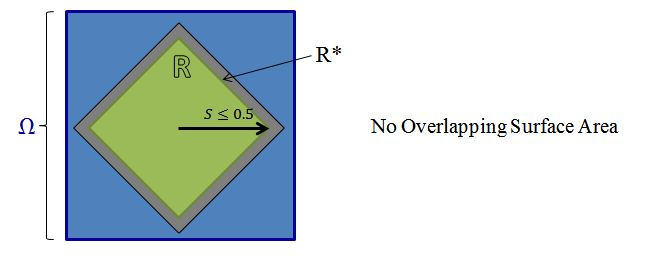
\includegraphics[scale=.6]{images/overlappingExplanation_1.jpg}
        \caption{$s \leq \frac{1}{2}$}
        \label{fig:first}
    \end{subfigure}
    \begin{subfigure}[b]{1\textwidth}
        \centering
        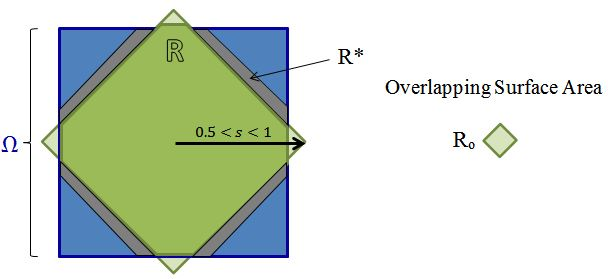
\includegraphics[scale=.6]{images/overlappingExplanation_2.jpg}
        \caption{$\frac{1}{2} < s < 1$. The gray region is the surface area of interest.}
        \label{fig:second}
    \end{subfigure}
    \begin{subfigure}[b]{1\textwidth}
        \centering
        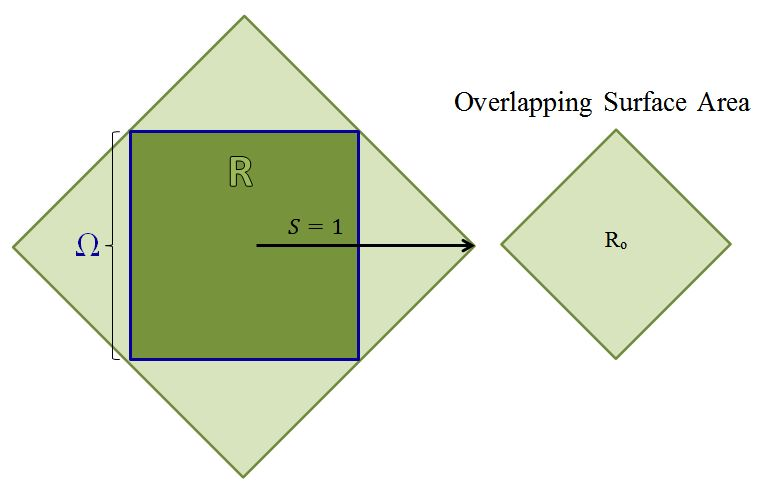
\includegraphics[scale=.5]{images/overlappingExplanation_3.jpg}
        \caption{$s = 1$}
        \label{fig:third}
    \end{subfigure}
    \caption{Illustration of $R$ for $D = 2$. For $s \leq \frac{1}{2}$ (a), the surface area of the cross polytope gives the desired surface area. For $\frac{1}{2} < s < 1$ (b) or $s = 1$ (c), the surface area of the cross polytope created by the overlapping area (shown on the right) must be subtracted.}
    \label{fig:examples}
\end{figure}

Even though the notion of surface area does not make sense in the one-dimensional case, this method still correctly predicts correct length of $R^*$. So, now we have
\begin{equation}
	A_{R}(s) = 
\begin{cases}
	A(\sqrt{2} s) & \mbox{if } s \leq \frac{1}{2} \\
   	A(\sqrt{2} s) - A\left(\frac{\sqrt{2}D}{D-1}\left(s-\frac{1}{2}\right)\right) & \mbox{if } s > \frac{1}{2}
\end{cases}
\end{equation}


Because $n$ vertices are spread evenly throughout the opinion space, the number of \emph{possible} edges $\{x, u\}$ such that $u \in R^*$ is 
$n \, A_{R}(s) \, \Delta s.$ And from Theorem \ref{thm:perc}, we know that the probability a specific one of these edges is present is $\frac{c}{s^2 + c}$. So, for specific vertex $x$, we expect there to be 
\begin{equation}
n\,A_{R^*}(s)\,\frac{c}{s^2 + c} \; \Delta s 
\end{equation}
 edges $\{x, u\}$ such that $s \leq d(x, u) \leq s + \Delta s.$ 

This argument can be repeated for every vertex $x$ in the graph; however, doing so will count each edge twice. Therefore the number of edges $e$ such that $s \leq d(e) \leq s + \Delta s$ is $\frac{n^2}{2}\,\frac{c}{s^2 + c}\,A_{R}(s) \; \Delta s $. When selecting a random edge, the probability that any given edge is selected is $\frac{1}{m}$. Thus $Pr(s \leq d(e) \leq s + \Delta s) = \frac{n^2}{2m}\,\frac{c}{s^2 + c}\,A_{R}(s) \; \Delta s $ for $\Delta s \to 0$.

By the definition of probability density function, 
\begin{equation}
 \int\limits_{s}^{s + \Delta s} \sigma(t)\,dt = Pr(s \leq d(e) \leq s + \Delta s).
\end{equation}
For $\Delta s \to 0$, the integral on the LHS is equal to $\sigma(s) \, \Delta s$. This gives us
 \begin{equation}
 \sigma(s) = \frac{n^2}{2m}\,\frac{c}{s^2 + c} A_{R}(s)
 \end{equation}
\end{proof}

\begin{figure}
 \centering
 	\begin{subfigure}[b]{.5\textwidth}
		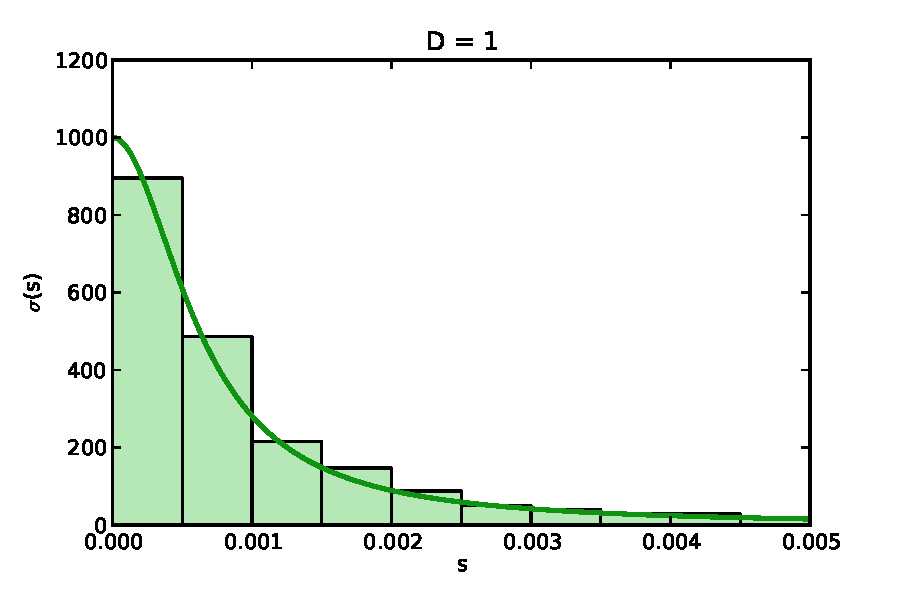
\includegraphics[scale=.45]{images/length_distro1.pdf}
 	\end{subfigure}
 	 \begin{subfigure}[b]{.4\textwidth}
		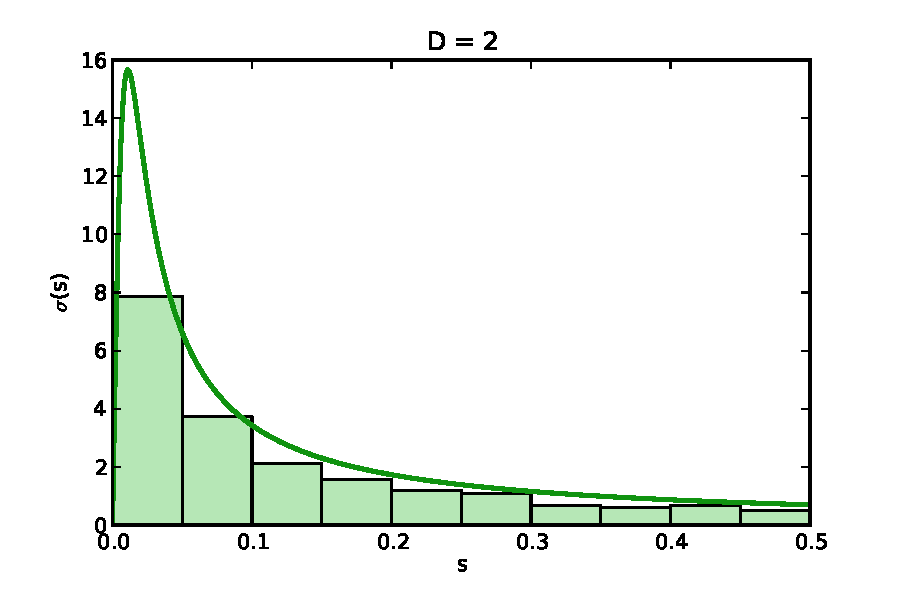
\includegraphics[scale=.45]{images/length_distro2.pdf}
 	\end{subfigure}
 	 \begin{subfigure}[b]{.4\textwidth}
		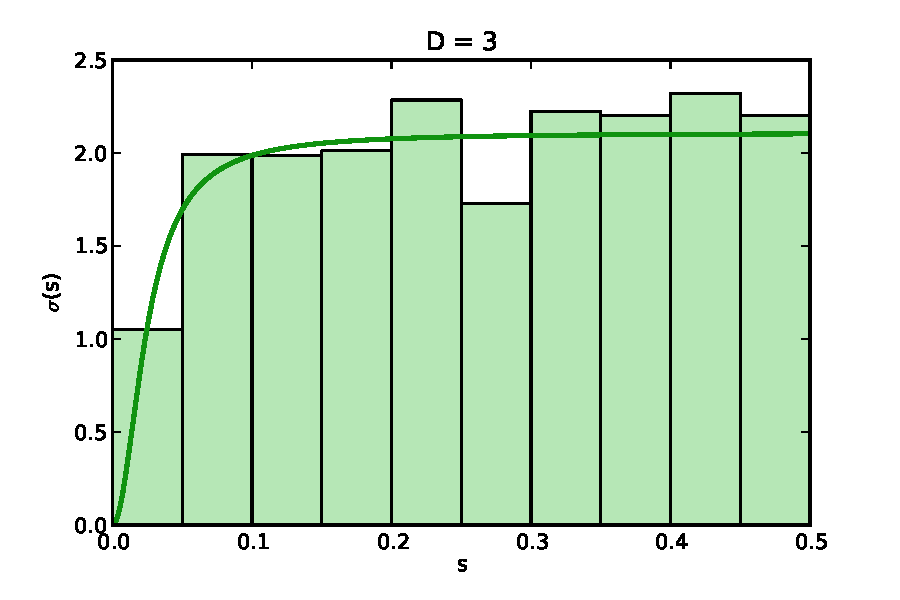
\includegraphics[scale=.45]{images/length_distro3.pdf}
 	\end{subfigure}
 \caption{The $\sigma(s)$ given by Theorem \ref{thm:length-distro} matchs experimental data. Data was collected using the constructive model. The graphs had 2000 vertices and mean degree 4. Note that the $D = 1$ plot has a different scale on the horizontal axis than the other two plots.}
\end{figure}

\begin{figure}
 \centering
 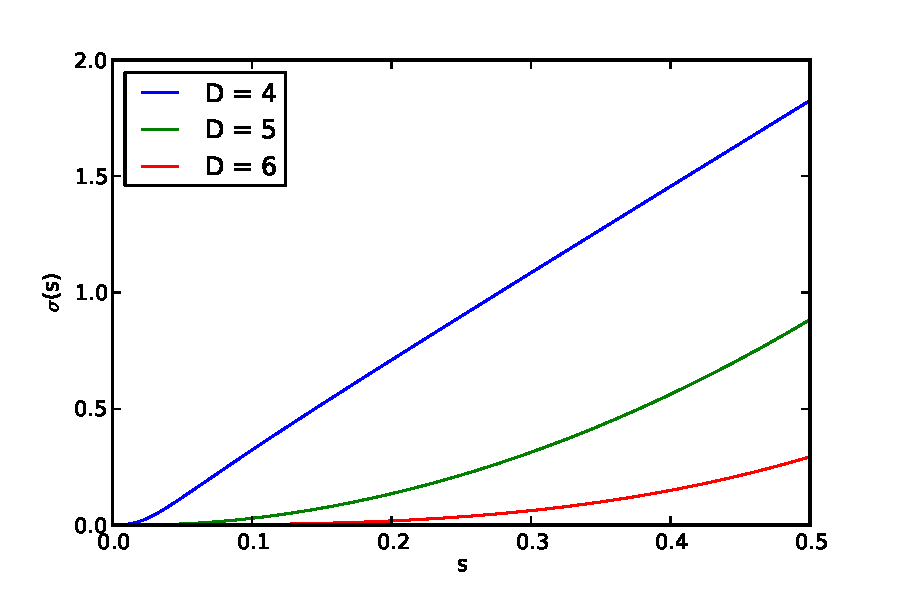
\includegraphics[scale=.7]{images/sigma_multi.pdf}
 \caption{Plot of $\sigma(s)$ for higher dimensions on graphs with 2000 vertices and mean degree 4. Theorem \ref{thm:length-distro} is not as useful for higher dimensions, as it only applies for $s \leq 1/2$ and edges can have length as great as $D$. }
\end{figure}

\section{Expected Degree}
\begin{theorem}
\label{thm:lambdax}
The expected degree of a vertex $x$ is
 \begin{equation}
 \lambda(x) = c\,n\int\limits_\Omega \frac{du}{d(x, u)^2 + c}.
\end{equation}
\end{theorem}
\begin{proof}
The expected number of vertices in an interval $I$ with dimensions $du_1, du_2, \ldots, du_D$  is $n \cdot du_1 \cdot du_2 \cdots du_D$ because $n$ vertices are evenly distrbuted within $\Omega$. From Theorem \ref{thm:perc}, we see that expected number of edges $\{x, u\}$ where $u \in I$ is $\frac{c}{d(x, u)^2 + c} \, n \, du$. Thus the expected degree of $x$ is this function integrated over $\Omega$.
\end{proof}

\begin{prop}
\label{prop:lambdax1}
For $D = 1$, The expected degree of a vertex $x = x_1$ is
 \begin{equation}
 \lambda(x) = n\sqrt{c}\left[\tan^{-1}\left(\frac{x}{\sqrt{c}}\right)+\tan^{-1}\left(\frac{1-x}{\sqrt{c}}\right)\right]
\end{equation}
\end{prop}
\begin{proof}
When $D=1$, Theorem \ref{thm:lambdax} reduces to
\begin{equation}
 \lambda(x) = c\,n\;\int\limits_{0}^{1} \frac{du}{(x - u)^2 + c}.
\end{equation}
Evaluating the integral yields our result.
\end{proof}

\begin{figure}
 \centering 
 	\begin{subfigure}[h]{1\textwidth}
 		\centering
 		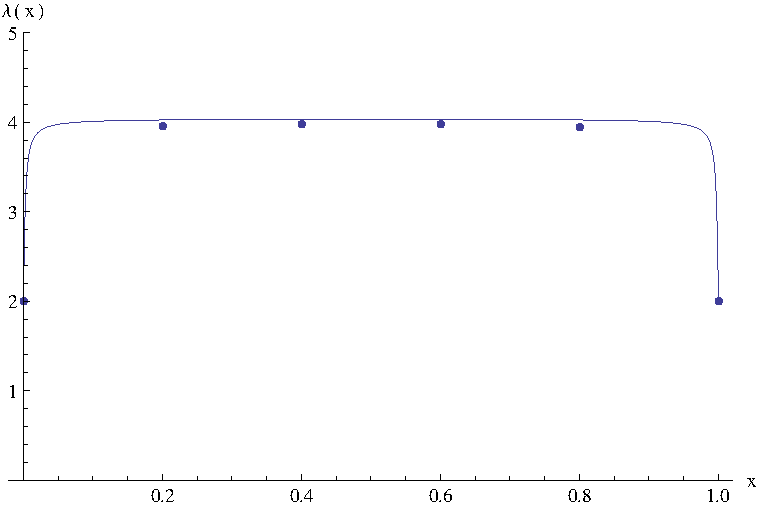
\includegraphics[scale=.85]{images/lambda_verify.pdf}
 		\caption{Experimental verification of Proposition \ref{prop:lambdax1} using data taken from the constructive model. The datapoints lie slightly below the curve; this is a side effect of the vertices being spaced evenly in the opinion space rather than placed randomly. The graph had 500 vertices. The coefficient $c$ was calculated using Proposition \ref{prop:c1D}.}
 	\end{subfigure}
 	\qquad
 	\begin{subfigure}[h]{1\textwidth}
 		\centering
 		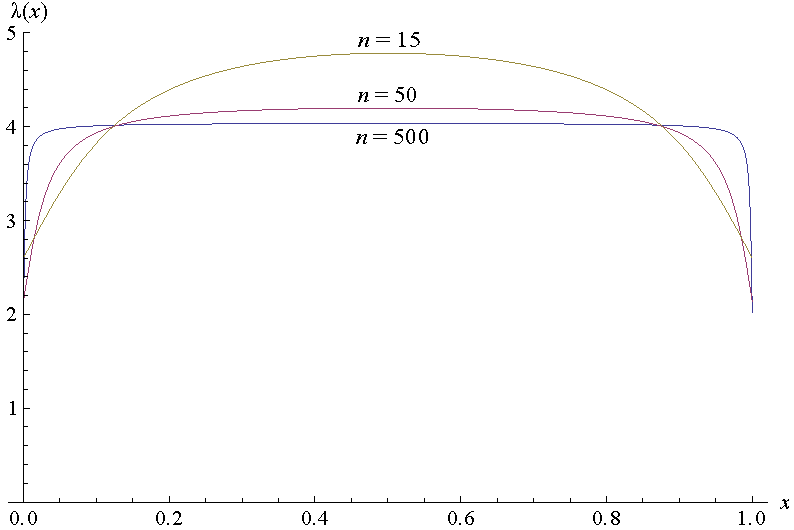
\includegraphics[scale=.85]{images/lambda_compare.pdf}
 		\caption{Comparison of $\lambda(x)$ for graphs of different sizes.}
 		\label{subfig:lambda-compare}
 	\end{subfigure}
 \caption{Plots of expected degree $\lambda$ vs. opinion $x$ in the one-dimensional case with mean degree 4. The curves have reflectional symmetry across $x = \frac{1}{2}$ as expected.}
 \label{fig:lambda}
\end{figure}

Figure \ref{fig:lambda} shows experimental verification of Proposition \ref{prop:lambdax1} --- and thus Theorem \ref{thm:lambdax} --- and a comparison of $\lambda(x)$ for graphs of different sizes. This second plot shows that, for reasonably large $n$, all vertices except those that are very close to the boundaries of the opinion space have $\lambda \approx \overline{k}$ where $\overline{k}$ is the mean degree. 

We posit that vertices $x$ such that $\min(x, 1 - x)$ is greater than the lengths of most edges have $\lambda \approx \overline{k}$; this is because almost none of the edges $\{x, u\}$ reach the boundary of the opinion space. On the other hand, vertices $x$ such that $\min(x, 1 - x)$ is not greater than the lengths of most edges have $\lambda < \overline{k}$ because the boundary of the opinion space prevents some edges $\{x, u\}$ that would otherwise be present. 

From Figure \ref{subfig:lambda-compare}, we see that the threshold $\min(x, 1 - x)$ at which $\lambda(x)$ begins to drop decreases with $n$. Table \ref{tbl:dist-distro} shows: first, that the mean edge distance seems to decrease as $n$ increases --- this is because, as vertices become more tightly-packed, shorter edges become possible --- and secondly, that the standard deviation from that mean also decreases as $n$ increases. These two facts explain why, for greater $n$, vertices can be closer to the boundary of the opinion space while still having $\lambda \approx \overline{k}.$

\begin{table}
\centering
\begin{tabular}{ c | c | c }
  $n$ & $\overline{d}$ & $\sigma$ \\ \hline
  15 & .16 & .14 \\
  50 & .042 & .058 \\
  500 & .0085 & .032 \\
\end{tabular}
\caption{Means and standard deviations of edge-distance distributions. Data was collected from the constructive model. The mean degree was 4.}
\label{tbl:dist-distro}
\end{table}

\newpage
\section{Degree Distribution}
The degree distribution of the vertices at equilibrium is Poisson.
\begin{proof}
Given a vertex with opinion $x$, the probability that this vertex is of degree $k$ is given by
	\begin{equation}
		p\left(deg(x)=k\right) = p(\{x, z\} \in E)^k (1 - p(\{x, z\} \in E))^{n-1-k}
	\end{equation}
where $p(\{x, z\} \in E)$ denotes the probability that a vertex of opinion $x$ is connected to a random vertex. This is equal to the total number of vertices that $x$ is connected to, divided by $n$. For large $n$, this is given by the equation
	\begin{equation}
		p(\{x, z\} \in E) = \frac{1}{n} \sum_{z \in V} \frac{n \cdot c}{d(x, z)^2 + c} = c \int\limits_\Omega \frac{dz}{d(v_x, z)^2 + c}
	\end{equation}
Using Equation 15, this is simply $\frac{\lambda(x)}{n}$. We know that for $x \ne 0^D, 1^D$, $\lambda(x)$ is some constant, so let $\frac{\lambda(x)}{n} = \eta$, for some constant $\eta$. We now have
	\begin{equation}
		p\left(deg(v_x)=k\right) = \eta ^k \left( 1 - \eta \right)^{n-1-k}
	\end{equation}
To get the unconditioned probability that a vertex has degree $k$, $p\left(deg(v)=k\right)$, we multiply by the condition that a vertex is of opinion $x$. Because vertices are randomly distributed, this is given by the constant $1/n$. Then, we sum it over all $n$ vertices.
	\begin{equation}
		p\left(deg(v)=k\right) =  \int\limits_\Omega \frac{1}{n} \cdot \eta ^k \left( 1 - \eta \right)^{n-1-k} n \ dx = \cdot \eta ^k \left( 1 - \eta \right)^{n-1-k}
	\end{equation}
	For large $n$, this is a Poisson distribution.
\end{proof}
\end{document}
